\PassOptionsToPackage{pdftex,
                        pdfauthor={Pavel Březina},
                        pdftitle={BP - Březina},
                        pdfsubject={Adaptivní přímovazební kompenzace statických sil působících na mechatronický systém}
                        }{hyperref}  
\documentclass[12pt, czech]{article}
% \raggedbottom
% \documentclass[12pt, czech]{article}
\usepackage[czech]{babel}

\usepackage{xstring}

\usepackage[T1]{fontenc} 
\usepackage[utf8]{inputenc}
\usepackage{lmodern}

\usepackage{float}
\usepackage{url}
\usepackage{graphicx}  % balík nutný pro vkládání obrázků
\usepackage{array}
\usepackage{amsmath}
\usepackage{siunitx}
\usepackage{enumitem}
\usepackage{microtype} % lepší zalomení textu
\usepackage{comment}
\usepackage{multirow}
\usepackage{geometry}
\usepackage{subcaption}
\usepackage[dvipsnames]{xcolor}
\usepackage{gensymb}
\usepackage{adjustbox}
\usepackage{placeins}
\usepackage{csvsimple}
\usepackage{mathtools}
\usepackage{etoolbox}
\usepackage{pgffor}
\usepackage{minted}
\usepackage{amssymb}
\usepackage{intcalc}
\usepackage{hyperref}
\hypersetup{
  colorlinks=true,
  linkcolor=RoyalBlue,
  citecolor=Red
  }
\usepackage[all]{hypcap}

\usepackage{pdfpages}
\usepackage{ifthen}

\usepackage{pdflscape}
\usepackage{fancyhdr}% http://ctan.org/pkg/fancyhdr
\usepackage{rotating}
\usepackage[autostyle]{csquotes}
\usepackage{multicol}
\usepackage{bm}
\usepackage{tikz}
\usepackage{attachfile2}

\usepackage{changepage} % check if page is odd or even
\usepackage{layout}
\usepackage[backend=biber,style=authortitle,]{biblatex}
\usepackage{titlesec}
\usepackage[stable]{footmisc} % \footnote in \section
\usepackage{animate}
\usepackage{parskip}

\usepackage{scrextend} % check if page is odd or even but better
\usepackage{afterpage}

\usepackage{csquotes}
\DeclareQuoteAlias{german}{czech}
\MakeOuterQuote{"}
\newenvironment{imagepage}{}{}
\BeforeBeginEnvironment{imagepage}{
  \newpage
  \newgeometry{top=0cm, bottom=0cm}
  \let\tmp\oddsidemargin
\let\oddsidemargin\evensidemargin
\let\evensidemargin\tmp
\reversemarginpar
  \begin{samepage}
    \vspace*{\fill}
    }
    \AfterEndEnvironment{imagepage}{
  \end{samepage}
  \vspace*{\fill}
  \restoregeometry}


\def\imagepageinnermargin{0cm}
\def\imagepageoutermargin{0cm}
\newenvironment{landscapeimagepage}{}{}
\BeforeBeginEnvironment{landscapeimagepage}{
  \newgeometry{top=0cm, bottom=0cm, left=0cm, right=0cm}
  \thispagestyle{empty}
  % \raggedright
  \newgeometry{top=0cm, bottom=0cm, left=\imagepageoutermargin, right=\imagepageinnermargin}
                % \ifthispageodd{\pagecolor{yellow}\afterpage{\nopagecolor}}
                % {\pagecolor{orange}\afterpage{\nopagecolor}}% I'm even
  % \checkoddpage
  % \ifoddpage odd%\newgeometry{top=0cm, bottom=0cm, left=\imagepageoutermargin, right=\imagepageinnermargin}
  % \else%\newgeometry{top=0cm, bottom=0cm, left=\imagepageinnermargin, right=\imagepageoutermargin}
  %   even
  % \fi
  % right je horní strana
  % \newgeometry{top=0cm, bottom=0cm, left=0cm, right=4cm}
  \begin{landscape}
    \thispagestyle{empty}
    % \ifthispageodd{I'm odd}{I'm even}% I'm even
    % \begin{samepage}
    % \vspace*{\fill}
    }
    \AfterEndEnvironment{landscapeimagepage}{
    % \vspace*{\fill}
    % \end{samepage}
  \end{landscape}
  % \raggedbottom
  \restoregeometry
  }

\newenvironment{nomargin}{}{}
\BeforeBeginEnvironment{nomargin}{
  \newgeometry{top=0cm, bottom=0cm, left=0cm, right=0cm}
  \vspace*{\fill}
}
\AfterEndEnvironment{nomargin}{
  \vspace*{\fill}
  \restoregeometry}

\setlength\parindent{0pt}

% https://tex.stackexchange.com/a/102845/255601
\newcommand{\todo}[1]{\textbf{\large{\textcolor{red}{#1}}}}

\newcommand*\centermathcell[1]{\omit\hfil$\displaystyle#1$\hfil\ignorespaces}

\newcommand{\subsubscheme}[2]{
  \begin{landscape}
    \thispagestyle{empty}
    \includepdf[pagecommand={\subsubsection{#1}\label{#1}},
      landscape=true,
      scale=0.95]{#2}
  \end{landscape}
}

\newcommand{\subscheme}[2]{
  \begin{landscape}
    \thispagestyle{empty}
    \includepdf[pagecommand={\subsection{#1}\label{#1}},
      landscape=true,
      scale=0.95]{#2}
  \end{landscape}
}

\newlist{enumerateabc}{enumerate}{1}
\setlist[enumerateabc]{label=\alph*.}

\DeclareMathOperator*{\argmax}{arg~max}
\DeclareMathOperator*{\argmin}{arg~min}
\DeclareMathOperator{\atantwo}{atan2}
\DeclareMathOperator{\diag}{diag}
\DeclareMathOperator{\imresize}{imresize}
\newcommand{\COV}[1]{\operatorname{COV}[#1]}
\newcommand{\E}[1]{\operatorname{E}[#1]}
\newcommand{\VAR}[1]{\operatorname{VAR}[#1]}

\DeclarePairedDelimiter\abs{\lvert}{\rvert}
\DeclarePairedDelimiter\norm{\lVert}{\rVert}

% https://tex.stackexchange.com/a/359261/255601
\let\olditem\item
\newcommand{\todoitem}{\let\item\olditem\color{red}\item\preto\item{\color{black}}}

\newcounter{numFrames}
\newboolean{stop}
\newcommand{\includeanimation}[3]{
  %\setcounter{numFrames}{-1} % fileName_0.pdf ... fileName_?.pdf
  \setcounter{numFrames}{0}
  \setboolean{stop}{false}
  \whiledo{\NOT\boolean{stop}}{
    \stepcounter{numFrames}
    \IfFileExists{#1\thenumFrames.png}{}{
      \addtocounter{numFrames}{-1}
      \setboolean{stop}{true}
    }
  }
  \begin{center}
    \shorthandoff{-}
    \animategraphics[autoplay, controls, loop, #3]{#2}{\detokenize{#1}}{0}{\thenumFrames}
    \shorthandon{-}
  \end{center}
}
\newcommand{\includeanimationframes}[3][]{
  \setcounter{numFrames}{0}
  \setboolean{stop}{false}
  \whiledo{\NOT\boolean{stop}}{
    \stepcounter{numFrames}
    \IfFileExists{#2\thenumFrames.png}{}{
      \addtocounter{numFrames}{-1}
      \setboolean{stop}{true}
    }
  }
  \foreach \n in {0,...,5}{
      % \n
      % \todo{\basiceval{\n*\thenumFrames/5}}
      \includegraphics[#3]{\detokenize{#2}\basiceval{\n*\thenumFrames/5}.png}
      \ifnum\n<3
        #1
      \fi
      \ifnum\intcalcMod{\intcalcInc{\n}}{3}=0
      \else
        \hspace{1cm}
      \fi
    }
}

\def\basiceval#1{\the\numexpr#1\relax}

\renewcommand*{\thefootnote}{[\arabic{footnote}]}

% ================================================================================================================
% https://tex.stackexchange.com/questions/60209/how-to-add-an-extra-level-of-sections-with-headings-below-subsubsection
% https://tex.stackexchange.com/a/60212
\makeatletter
\renewcommand\paragraph{\@startsection{paragraph}{4}{\z@}%
  {-2.5ex\@plus -1ex \@minus -.25ex}%
  {1.25ex \@plus .25ex}%
  {\normalfont\normalsize\bfseries}}
\makeatother
\setcounter{secnumdepth}{4} % how many sectioning levels to assign numbers to
\setcounter{tocdepth}{4}    % how many sectioning levels to show in ToC
% ================================================================================================================
\makeatletter
\newcommand\footnoteref[1]{\protected@xdef\@thefnmark{\ref{#1}}\@footnotemark}
\makeatother

% ================================================================================================================


\usetikzlibrary{shapes,arrows,positioning,calc}

\newboolean{includeAnimations}
\setboolean{includeAnimations}{false}

\newboolean{includeAnimationFrames}
\setboolean{includeAnimationFrames}{true}

\setcounter{tocdepth}{3}    % how many sectioning levels to show in ToC

% pro tisk
% \def\imagepageinnermargin{2cm}
% \def\imagepageoutermargin{0.5cm}

\def\imagepageinnermargin{1cm}
\def\imagepageoutermargin{1cm}

% \newcommand{\getmode}{dark-mode}

% \ifthenelse{\equal{\getmode}{dark-mode}}
%     {% true
%       \pagecolor[rgb]{0,0,0}
%       \color[rgb]{0.95,0.95,0.95}
%     }
\addbibresource{Reference.bib}

\begin{document}
\pagenumbering{gobble}
\begin{center}
    
\includegraphics[height=0.21\textheight]{Img/FAV_logo.pdf}
    
\includegraphics[height=0.21\textheight]{Img/zcu-logo.pdf}
\end{center}
\begin{center}
    \vspace{3cm}
    % \textbf{\LARGE{NURBS spliny pro modelování křivek a povrchů a jejich použití v robotice}}\\
    \LARGE{NURBS spliny pro modelování křivek a povrchů a jejich použití v robotice}
\end{center}
\vfill{}
\noindent
Západočeská Univerzita V Plzni \hfill Pavel Březina\\
Katedra Kybernetiky            \hfill letní semestr\\
PAŘR5                \hfill \today
\thispagestyle{empty}
\newpage
\thispagestyle{empty}
\tableofcontents
\newpage
\listoffigures
\null\newpage

\pagenumbering{arabic}
\section{Úvod}
V práci je nejprve popsána struktura řídících smyček pohybu lékařského CT manipulátoru Phillips Azurion 7 C20
včetně proudové kalibrační tabulky (CCT). Kalibrační tabulka hraje zásadní roli pro dosažení přesných pohybů jednotlivých kloubů a~zajištění přesného a~konzistentního chování při lékařských zákrocích. Z~důvodu přirozeného opotřebení stroje je však nutná pravidelná rekalibrace, která vede k~nežádoucím odstávkám. Cílem této práce je proto navrhnout řešení, jak minimalizovat potřebu rekurentních manuálních rekalibrací stroje pomocí vhodného algoritmu aktualizace CCT, čímž by se zvýšila přesnost a~spolehlivost manipulátoru a~také snížil počet odstávek stroje.
\par
Tato práce se zabývá řešením pomocí B-spline interpolace/aproximace. Interpolace a~aproximace jsou rozhodujícími technikami pro problém aktualizace CCT, které umožňují vyvodit správné hodnoty v~bodech ležících mimo síť naměřených bodů v~této tabulce.\par
% Navrhované řešení by mohlo výrazně zlepšit proces kalibrace, což by v~konečném důsledku vedlo ke spolehlivějšímu a 
Text je rozdělen na několik hlavních částí:
\begin{enumerate}
    \item \nameref{section: řízený a~říddící systém} --- část zaměřená na řízený a~řídící systém, která obsahuje technické specifikace robota, popis problému a~také zvolený přístup řešení
    \item \nameref{section: NURBS teorie} --- obsáhlá kapitola, ve které je rozebrána veškerá teorie k~NURBS křivkám/povrchům včetně kompletně vlastní implementace v~Matlabu dle knihy \cite{The_NURBS_Book}. Kapitola obsahuje ukázky výsledků jednotlivých algoritmů na obecných datech.
    \item \nameref{section: návrh automatické kalibraci} --- část, ve které jsou vizualizovány výsledky aplikace principů NURBS teorie na reálných datech. Dále v~této kapitole byly také využity techniky z~oblasti zpracování signálů, za účelem nalezení vhodných částí měření, které by se daly využít pro aktualizaci CCT.
\end{enumerate}
Všechny hodnoty poloh a~proudů pro jednotlivé klouby byly v~práci znormovány tak, aby bylo omezeno riziko úniku citlivých dat společnosti Phillips. Jedná se tak o~bezrozměrné veličiny, u~kterých nejsou uvedeny jednotky.
\par
V~případě ukázky animací je zobrazeno pouze 6 snímků pro tištěnou verzi, plná verze animace je obsažena v~příloze či v~digitální verzi dokumentace. Celá tato práce včetně zdrojového kódu je veřejně dostupná online --- \cite{Github}.
% \begin{imagepage}
% https://www.philips.cz/healthcare/product/HCNCVD207/azurion-7-c20-with-flexarm-image-guided-therapy-system
% https://www.philips.de/c-dam/corporate/newscenter/de/press-releases/2019/20190122-azurion-7-c20-mit-flexarm/philips-azurion-7-c20-mit-flexarm-produkt2-un-hs-20190122.download.jpg
\begin{figure}[H]
    \centering
    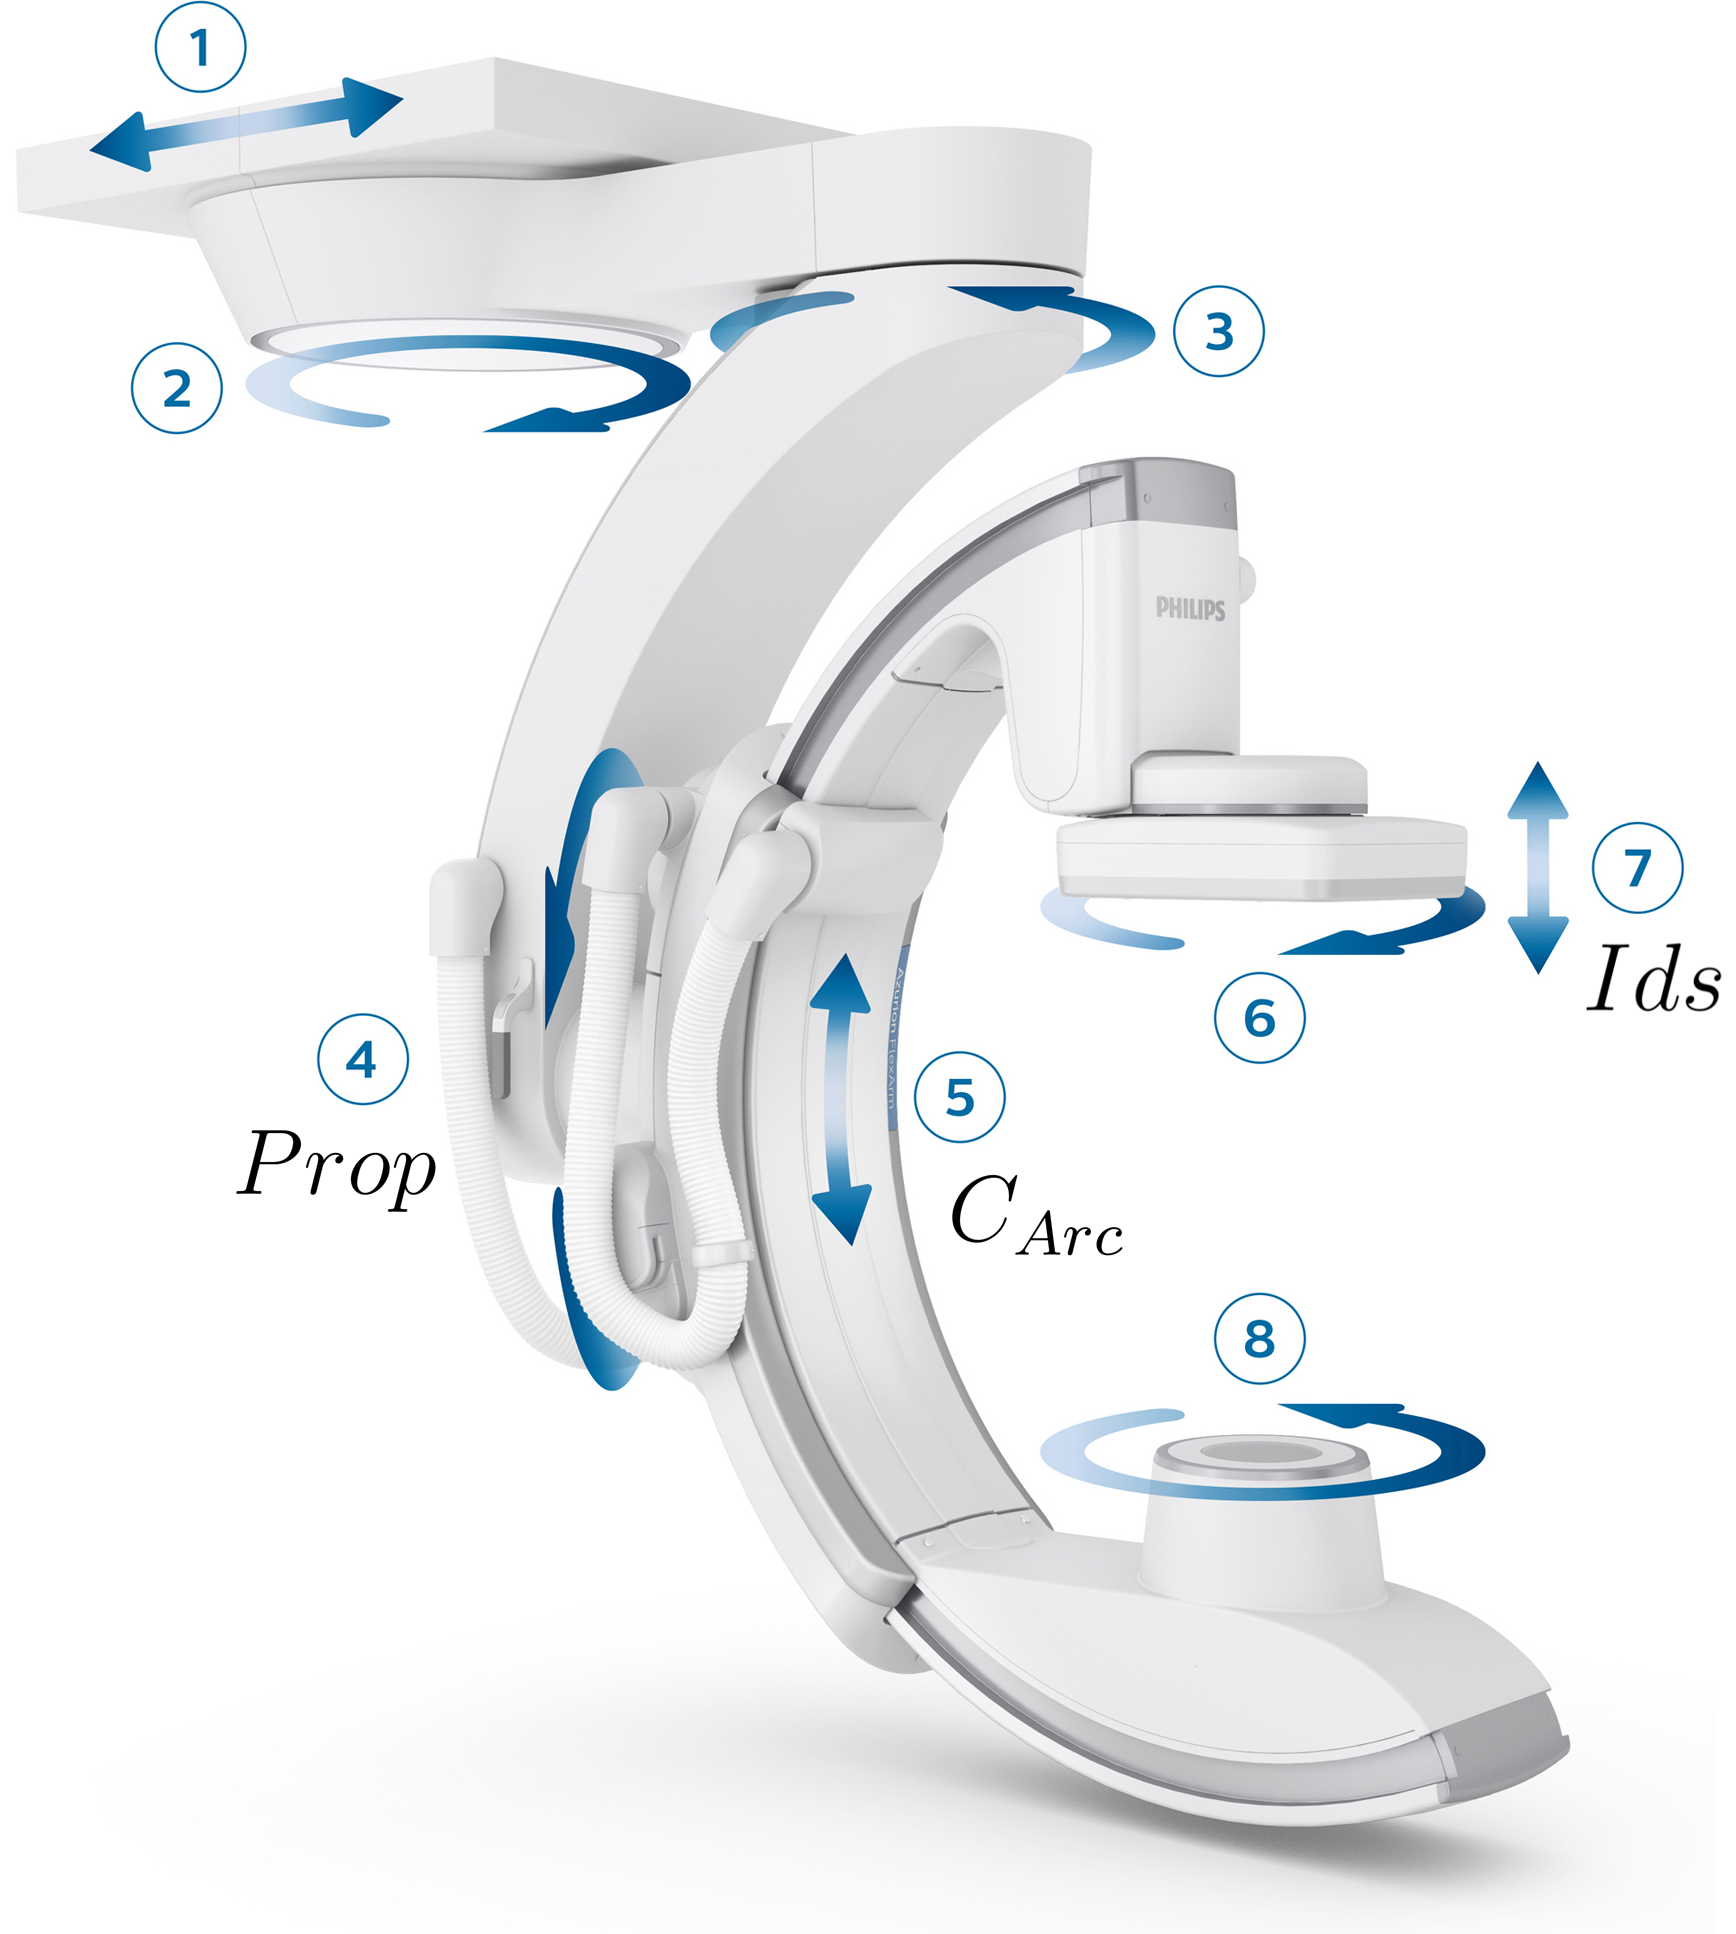
\includegraphics[width=\textwidth]{Img/Azurion 7 C20 with FlexArm modified.png}
    \caption[Výpočetní tomograf s~8 stupni volnosti Phillips Azurion 7 C20]{Výpočetní tomograf s~8 stupni volnosti Phillips Azurion 7 C20 --- \cite{Azurion}}
    \label{fig:Výpočetní tomograf}
\end{figure}
% \end{imagepage}
\section{NURBS teorie}\label{section: NURBS teorie}
Tato kapitola je zaměřena na algoritmy pro práci s NURBS křivkami/povrchy, které jsou ručně implementovány v Matlabu podle knížky \cite{The_NURBS_Book}. V každé podkapitole je uveden odpovídající zdroj z této knížky. Implementace těchto algoritmů je nezbytná pro realizaci autonomní rekalibrace CCT dle návrhu uvedeného v předchozích kapitolách.
% \par
% V kapitole se hojně užívá pojmů ``interpolace'' a ``aproximace'', popřípadě ještě ``extrapolace'', zde je vysvětlení těchto pojmů:
% \begin{itemize}
%     \item Interpolace --- Hledání spojité funkce, jejichž funkční hodnoty odpovídají námi zadaným hodnotám na příslušných souřadnicích. Existuje mnoho interpolačních metod například: lineární interpolace, kosinové interpolace, kubická interpolace a polynomiální interpolace. Zejména polynomiální interpolace není pro naše účely vhodná, protože pro velké množství bodů nabývá vysokého řádu a má tendenci kmitat, toto obzvlášť platí pro ekvidistantně zadané interpolační body.
%     \item Aproximace --- Hledání spojité funkce, která nějakým vhodným způsobem pro danou úlohu nejlépe popisuje aproximační body. Pro naše účely budeme používat NURBS aproximaci založenou na vážené metodě nejmenších čtverců. Tento přístup nám umožní volit stupeň polynomu bázových funkcí, míru redukce bodů (pomocí počtu řídících bodů) a také váhy jednotlivých bodů.
%     \item Extrapolace --- Využití interpolované/aproximované funkce mimo původní rozsah interpolačních/aproximačních bodů. Přesnost extrapolace závisí na charakteru zvolené interpolační/aproximační metody a zdrojových dat. V této práci se extrapolace nevyužívá, protože jí není potřeba, a také proto, že NURBS metodu nelze pro extrapolaci použít.
% \end{itemize}
\subsection[NURBS křivky]{NURBS křivky \footcite[kapitola 3.2]{The_NURBS_Book}}\label{section: NURBS křivky}
Neuniformní racionální B-spline (NURBS) křivku $\bm{C}(u)$\footnote{Jedná se tedy o vektorovou funkci skalární proměnné.} definujeme následovně:
\begin{equation}
    \bm{C}(u) = \sum_{i = 0}^{n} N_{i, p}(u)\bm{P}_i\quad a\le u \le b
\end{equation}
kde
\begin{itemize}
    \item $p$ značí stupeň křivky
    \item $n$ značí počet řídících bodů
    \item $\bm{P}_i$ jsou řídící body, $\dim{\bm{P}_i} \ge 2$
    \item parametry $a$ a $b$ lze znormovat bez ztráty obecnosti --- nejčastěji se udávají hodnoty
          $a = 0$, $b = 1$, které budeme též používat
    \item $N_{i,p}$ jsou B-spline bázové funkce stupně $p$ definované
          na neperiodickém neekvidistantním uzlovém vektoru $\bm{U}$
    \item $u \in \bm{U}$
\end{itemize}
Pro uzlový vektor $\bm{U}$ platí:
\begin{equation}
    \bm{U} = \{\overbrace{\underbrace{a, \ldots, a}_{p + 1}, u_{p + 1}, \ldots, u_{m -p - 1}, \underbrace{b, \ldots, b}_{p + 1}}^{m + 1}\}
\end{equation}
kde $m = n + p + 1$.\par
Bázové funkce lze definovat rekurzivně (výhoda jednoduché implementace):
\begin{align}
    N_{i,0}(u)  & = \begin{cases}
                        1 \quad u_i \le u < u_{i + 1} \\
                        0 \quad jinak
                    \end{cases}                \nonumber         \\
    N_{i, p}(u) & = \frac{u - u_i}{u_{i + p} - u_i}N_{i,p- 1}(u)
    + \frac{u_{i + p + 1} - u}{u_{i + p + 1} - u_{i + 1}}N_{i + 1, p - 1}(u)\label{eq:bázová funkce}
\end{align}
\subsection[NURBS povrchy]{NURBS povrchy\footcite[kapitola 3.4]{The_NURBS_Book}}
Pro sestrojení NURBS povrchu potřebujeme obousměrnou síť řídících bodů $\bm{P}_{i,j}$ a
dva uzlové vektory $\bm{U}$ a $\bm{V}$, poté je možné sestrojit povrch $\bm{S}(u,v)$\footnote{Jedná se tedy o vektorovou funkci dvou skalárních proměnných.}:
\begin{align}
    \bm{S}(u,v) = \sum_{i=0}^{n}\sum_{j=0}^{m}N_{i,p}(u)N_{j,q}(v)\bm{P}_{i,j}
\end{align}
kde
\begin{itemize}
    \item $p$ značí stupeň křivek ve směru $u$
    \item $q$ značí stupeň křivek ve směru $v$
    \item $n$ značí počet řídících bodů ve směru $u$
    \item $m$ značí počet řídících bodů ve směru $v$
    \item $\bm{P}_{i,j}$ je síť řídících bodů, $\dim{\bm{P}_{i,j}} \ge 3$
    \item $u \in \bm{U}$, $v \in \bm{V}$
    \item $a \le u \le b$, $a \le v \le b$ --- stejně jako u \nameref{section: NURBS křivky} budeme uvažovat $a = 0$, $b = 1$ bez ztráty obecnosti
\end{itemize}
Pro uzlové vektory $\bm{U}$ a $\bm{V}$ platí:
\begin{align}
    \bm{U} = \{\overbrace{\underbrace{a, \ldots, a}_{p + 1}, u_{p + 1}, \ldots, u_{r -p - 1}, \underbrace{b, \ldots, b}_{p + 1}}^{r + 1}\}\\
    \bm{V} = \{\overbrace{\underbrace{a, \ldots, a}_{q + 1}, u_{q + 1}, \ldots, u_{s -q - 1}, \underbrace{b, \ldots, b}_{q + 1}}^{s + 1}\}
\end{align}
kde $r = n + p + 1$, $s = m + q + 1$. \par Definice bázových funkcí zůstává stejná --- viz (\ref{eq:bázová funkce}).
\subsection[NURBS interpolace křivky]{NURBS interpolace křivky\footcite[kapitola 9.2.1]{The_NURBS_Book}}\label{section: interpolace křivky}
Mějme množinu $n + 1$ bodů $\{\bm{Q}_k\}$ $k = 0, \ldots, n$, které chceme
interpolovat NURBS křivkou stupně $p$. Pokud každému bodu $\bm{Q}_k$ přiřadíme
parametr $\bar{u}_k$, a vhodně sestrojíme uzlový vektor $\bm{U} = \{u_0, \ldots,
    u_m\}$, můžeme sestavit soustavu lineárních rovnic o rozměru $(n + 1)\times(n +
    1)$:
\begin{equation}
    \bm{Q}_k = \bm{C}(\bar{u}_k) = \sum_{i = 0}^{n}N_{i,p}(\bar{u}_k)\bm{P}_i
\end{equation}
kde řídící body $\bm{P}_i$ tvoří našich $n + 1$ neznámých.\par
Parametr $\bar{u}_k$ lze zvolit více způsoby, z nichž jsou běžné například:
\begin{itemize}
    \item ekvidistantní (equally spaced):
          \begin{alignat}{3}
              \bar{u}_0 & = 0           \quad\quad & \bar{u}_n & =1                 \\
              \bar{u}_k & = \frac{k}{n} \quad\quad & k         & = 1, \ldots, n - 1
          \end{alignat}
          Tato metoda je vhodná pro rovnoměrně rozprostřená data.
    \item délka tětivy (chord length) --- nechť $d$ je celková délka tětivy:
          \begin{equation}
              d = \sum_{k = 1}^{n}\norm{\bm{Q}_k - \bm{Q}_{k - 1}}
          \end{equation}
          potom
          \begin{equation}
              \bar{u}_0 = 0 \quad\quad \bar{u}_n = 1\\
          \end{equation}
          \begin{equation}
              \bar{u}_k = \bar{u}_{k - 1} + \frac{\norm{\bm{Q}_k - \bm{Q}_{k - 1}}}{d}
              \quad\quad k=1,\ldots,n-1
              \label{eq:chord length}
          \end{equation}
          Tato metoda je vhodná pro obecná data.
    \item dostředivá metoda (centripetal method) --- nechť $d$:
          \begin{equation}
              d = \sum_{k = 1}^{n}\sqrt{\norm{\bm{Q}_k - \bm{Q}_{k - 1}}}
          \end{equation}
          potom
          \begin{equation}
              \bar{u}_0 = 0 \quad\quad \bar{u}_n = 1\\
          \end{equation}
          \begin{equation}
              \bar{u}_k = \bar{u}_{k - 1} + \frac{\norm{\bm{Q}_k - \bm{Q}_{k - 1}}}{d}
              \quad\quad k=1,\ldots,n-1
              \label{eq:centripetal method}
          \end{equation}
          Tato metoda je vhodná pro obecná data s náhlými změnami směru.
\end{itemize}
Pro tyto metody je doporučený způsob výpočtu $\bm{U}$ metodou průměrování:
\begin{alignat}{3}
    u_0     & = \ldots = u_p = 0 \quad\quad                      & u_{m-p} & = \ldots = u_m = 1 \nonumber                             \\
    u_{j+p} & =\frac{1}{p}\sum_{i=j}^{j+p-1}\bar{u}_1 \quad\quad & j       & =1,\ldots, n -p    \label{eq:uzlový vektor průměrováním}
\end{alignat}
Nyní můžeme sestavit matici $\bm{N}$ $(n + 1) \times (n + 1)$:
\begin{equation}
    \bm{N} = \begin{bmatrix}
        N_{0,p}(\bar{u}_0)        & \cdots & N_{n+1,p}(\bar{u}_0)       \\
        \vdots                    & \ddots & \vdots                     \\
        N_{0, p}(\bar{u}_{n + 1}) & \cdots & N_{n+1,p}(\bar{u}_{n + 1})
    \end{bmatrix}
\end{equation}
Hledané řídící body $\bm{P}$ již spočteme vyřešením soustavy linárních rovnic:
\begin{align}
    \bm{P} = \bm{N}^{-1}\bm{Q}
\end{align}
Takto zavedená interpolace funguje pro libovolnou dimenzi bodů $\bm{Q}_k$.

\subsubsection{Ukázka 2D interpolace}
Na obrázku č. \ref{fig:Demo interpolace 2D} jsou porovnány zmíněné algoritmy
výpočtu parametru $\bar{u}_k$ pro tyto body:
\begin{equation}
    \bm{Q}_k = \begin{bmatrix}
        \bm{x} & \bm{y}
    \end{bmatrix}
    =\input{Generated/Interpolační body demo 2D.tex}
\end{equation}

\subsubsection{Ukázka 3D interpolace}
Na obrázku č. \ref{fig:Demo interpolace 3D} jsou porovnány zmíněné algoritmy
výpočtu parametru $\bar{u}_k$ pro tyto body:
\begin{equation}
    \bm{Q}_k = \begin{bmatrix}
        \bm{x} & \bm{y} & \bm{z}
    \end{bmatrix}
    =\input{Generated/Interpolační body demo 3D.tex}
\end{equation}

\begin{imagepage}
    \begin{figure}[H]
        \centering
        \includegraphics[width=0.85\textwidth]{Generated/Demo interpolace křivky 2D.pdf}
        \caption{Porovnání algoritmů interpolace ve 2D}
        \label{fig:Demo interpolace 2D}
    \end{figure}
    \begin{figure}[H]
        \centering
        \includegraphics[width=0.85\textwidth]{Generated/Demo interpolace křivky 3D.pdf}
        \caption{Porovnání algoritmů interpolace ve 3D}
        \label{fig:Demo interpolace 3D}
    \end{figure}
\end{imagepage}
% \subsection{Interpolace 4D křivky}
Interpolací 4D křivky je v tomto případě myšlena křivka tvořena 3D body ($x, y,
    z$), které se mění v závislosti na 4. souřadnici $w$. Tudíž nechceme
interpolovat jednu dlouhou 4D křivku (jak jsme dosud dělali v předchozích
případech), ale vlastně několik 3D křivek mezi sebou za využití 4.
souřadnice.\par Tohoto docílíme interpolací samotných bodů příslušných křivek
přes souřadnici $w$, kterou lze vidět na obrázcích č. \ref{fig:Demo 4D
    Interpolace mezi body přes souřadnici w 1}, \ref{fig:Demo 4D Interpolace mezi
    body přes souřadnici w 2}, \ref{fig:Demo 4D Interpolace mezi body přes
    souřadnici w 3}. Dále obrázky č. \ref{fig:Demo 4D Interpolace mezi body přes
    souřadnici w shora 1}, \ref{fig:Demo 4D Interpolace mezi body přes souřadnici w
    shora 2} a \ref{fig:Demo 4D Interpolace mezi body přes souřadnici w shora 3}
značí pohled na přechodové křivky shora, a obrázky č. \ref{fig:Demo 4D
    Interpolace mezi body přes souřadnici w konst x 1}, \ref{fig:Demo 4D
    Interpolace mezi body přes souřadnici w konst x 2} a \ref{fig:Demo 4D
    Interpolace mezi body přes souřadnici w konst x 3} ukazují interpolaci mezi
jedním bodem z každé křivky.

\subsubsection{4D Křivka číslo 1}
Tuto 4D křivku tvoří tři 3D křivky popsané body:
\begin{alignat}{3}
    \bm{Q}_1 & = [\bm{x}, \bm{y}, \bm{z}, \bm{w}] & = & [\bm{x}, \sin(\bm{x}), 10, 0]   \\
    \bm{Q}_2 & = [\bm{x}, \bm{y}, \bm{z}, \bm{w}] & = & [\bm{x}, -\sin(\bm{x}), 0, 100] \\
    \bm{Q}_3 & = [\bm{x}, \bm{y}, \bm{z}, \bm{w}] & = & [\bm{x}, \sin(\bm{x}), 20, 200]
\end{alignat}
kde
\begin{equation}
    \bm{x} = linspace(0, 2\cdot\pi, 25)
\end{equation}
Tyto fáze naší 4D křivky jsou rovnoměrně rozmístěny ve 4. dimenzi, tj.
$\bm{w}$ = $0, 100, 200$ při křivky 1, 2 a 3 respektive. Tímto by přechod mezi křivkami měl
být \todo{rovnoměrný? plynulý? symetrický?}. Ukázka přechodu mezi těmito křivkami je
zobrazena na animaci č. \ref{fig:Demo 4D Interpolace mezi křivkami č. 1}.
\subsubsection{4D Křivka číslo 2}
Tuto 4D křivku tvoří tři 3D křivky popsané body:
\begin{alignat}{3}
    \bm{Q}_1 & = [\bm{x}, \bm{y}, \bm{z}, \bm{w}] & = & [\bm{x}, \sin(\bm{x}), 10, 0]                            \\
    \bm{Q}_2 & = [\bm{x}, \bm{y}, \bm{z}, \bm{w}] & = & [\bm{x}, -\sin(\bm{x}), 0, \text{\textcolor{red}{$50$}}] \\
    \bm{Q}_3 & = [\bm{x}, \bm{y}, \bm{z}, \bm{w}] & = & [\bm{x}, \sin(\bm{x}), 20, 200]
\end{alignat}
kde
\begin{equation}
    \bm{x} = linspace(0, 2\cdot\pi, 25)
\end{equation}
V tomto případě interpolační křivky již nejsou rozmístěny rovnoměrně ve 4. dimenzi,
což v našem případě znamená, že přechod od křivky tvořenou body $\bm{Q}_1$ do křivky
tvořenou $\bm{Q}_2$ je $4\times$ kratší, než přechod od $\bm{Q}_2$ do $\bm{Q}_3$. Toto
je naznačené na obrázcích č.~\ref{fig:Demo 4D Interpolace mezi body přes souřadnici w 2},
\ref{fig:Demo 4D Interpolace mezi body přes souřadnici w shora 2} a
\ref{fig:Demo 4D Interpolace mezi body přes souřadnici w konst x 2},
kde je nepoměr vidět (přestože je zkreslený).
Pořádně lze tento jev vidět až na animaci č. \ref{fig:Demo 4D Interpolace mezi křivkami č. 2},
kde je také celý průběh interpolace.

\subsubsection{4D Křivka číslo 3}
Tuto 4D křivku tvoří tři 3D křivky popsané body:
\begin{alignat}{3}
    \bm{Q}_1 & = [\bm{x}, \bm{y}, \bm{z}, \bm{w}] & = & [\bm{x}, \sin(\bm{x}), 10, 0]                        \\
    \bm{Q}_2 & = [\bm{x}, \bm{y}, \bm{z}, \bm{w}] & = & [\bm{x}, -\sin(\bm{x}), 2.5 + 2.5\cos(2\bm{x}), 100] \\
    \bm{Q}_3 & = [\bm{x}, \bm{y}, \bm{z}, \bm{w}] & = & [\bm{x}, \sin(\bm{x}), 17.5 - 2.5\cos(2\bm{x}), 200]
\end{alignat}
kde
\begin{equation}
    \bm{x} = linspace(0, 2\cdot\pi, 25)
\end{equation}
Zde se pro ukázku interpolované křivky mění i v ose $z$ v závislosti na $x$.
Obrázky k této interpolaci jsou \ref{fig:Demo 4D Interpolace mezi body přes souřadnici w 3},
\ref{fig:Demo 4D Interpolace mezi body přes souřadnici w shora 3},
\ref{fig:Demo 4D Interpolace mezi body přes souřadnici w konst x 3} a
\ref{fig:Demo 4D Interpolace mezi křivkami č. 3}.

\begin{imagepage}
    \begin{figure}[H]
        \centering
        \includegraphics[height=0.4\textheight]{Generated/Interpolace 4D křivky - Interpolace mezi body ve 4. dimenzi č. 1.pdf}
        \caption{Interpolace bodů křivek přes souřadnici $w$ č. 1}
        \label{fig:Demo 4D Interpolace mezi body přes souřadnici w 1}
    \end{figure}
    \begin{figure}[H]
        \centering
        \includegraphics[height=0.4\textheight]{Generated/Interpolace 4D křivky - Interpolace mezi body ve 4. dimenzi (shora) č. 1.pdf}
        \caption{Interpolace bodů křivek přes souřadnici $w$ (pohled shora) č. 1}
        \label{fig:Demo 4D Interpolace mezi body přes souřadnici w shora 1}
    \end{figure}
\end{imagepage}

\begin{imagepage}
    \begin{figure}[H]
        \centering
        \includegraphics[height=0.4\textheight]{Generated/Interpolace 4D křivky - Interpolace mezi body ve 4. dimenzi 1 vlákno č. 1.pdf}
        \caption{Ukázka interpolace pro 1 bod z každé křivky č. 1}
        \label{fig:Demo 4D Interpolace mezi body přes souřadnici w konst x 1}
    \end{figure}
    \ifthenelse{\boolean{includeAnimations}}{
        \begin{figure}[H]
            \centering
            \includeanimation{Generated/4D curve demo 1/frame-}{12.5}{palindrome, height=0.4\textheight}
            \caption{Ukázka průběhu interpolace mezi křivkami přes souřadnici $w$ č. 1}
            \label{fig:Demo 4D Interpolace mezi křivkami č. 1}
        \end{figure}
    }{}
\end{imagepage}
\ifthenelse{\boolean{includeAnimationFrames}}{
    \begin{landscapeimagepage}
        \vspace*{\fill}
        \begin{figure}[H]
            \centering
            \includeanimationframes[\vspace{1cm}]{Generated/4D curve demo 1/frame-}{width=0.28\pdfpageheight}
            \caption{Ukázka průběhu interpolace mezi křivkami přes souřadnici $w$ č. 1}
            \label{fig:Demo 4D Interpolace mezi křivkami č. 1}
        \end{figure}
        \vspace*{\fill}
    \end{landscapeimagepage}}{}
% ======================================
\begin{imagepage}
    \begin{figure}[H]
        \centering
        \includegraphics[height=0.4\textheight]{Generated/Interpolace 4D křivky - Interpolace mezi body ve 4. dimenzi č. 2.pdf}
        \caption{Interpolace bodů křivek přes souřadnici $w$ č. 2}
        \label{fig:Demo 4D Interpolace mezi body přes souřadnici w 2}
    \end{figure}
    \begin{figure}[H]
        \centering
        \includegraphics[height=0.4\textheight]{Generated/Interpolace 4D křivky - Interpolace mezi body ve 4. dimenzi (shora) č. 2.pdf}
        \caption{Interpolace bodů křivek přes souřadnici $w$ (pohled shora) č. 2}
        \label{fig:Demo 4D Interpolace mezi body přes souřadnici w shora 2}
    \end{figure}
\end{imagepage}

\begin{imagepage}
    \begin{figure}[H]
        \centering
        \includegraphics[height=0.4\textheight]{Generated/Interpolace 4D křivky - Interpolace mezi body ve 4. dimenzi 1 vlákno č. 2.pdf}
        \caption{Ukázka interpolace pro 1 bod z každé křivky č. 2}
        \label{fig:Demo 4D Interpolace mezi body přes souřadnici w konst x 2}
    \end{figure}
    \ifthenelse{\boolean{includeAnimations}}{
        \begin{figure}[H]
            \centering
            \ifthenelse{\boolean{includeAnimations}}{\includeanimation{Generated/4D curve demo 2/frame-}{12.5}{palindrome, height=0.4\textheight}}{}
            \caption{Ukázka průběhu interpolace mezi křivkami přes souřadnici $w$ č. 2}
            \label{fig:Demo 4D Interpolace mezi křivkami č. 2}
        \end{figure}
    }{}
\end{imagepage}
\ifthenelse{\boolean{includeAnimationFrames}}{
    \begin{landscapeimagepage}
        \vspace*{\fill}
        \begin{figure}[H]
            \centering
            \includeanimationframes[\vspace{1cm}]{Generated/4D curve demo 2/frame-}{width=0.28\pdfpageheight}
            \caption{Ukázka průběhu interpolace mezi křivkami přes souřadnici $w$ č. 2}
            \label{fig:Demo 4D Interpolace mezi křivkami č. 2}
        \end{figure}
        \vspace*{\fill}
    \end{landscapeimagepage}}{}
% =====================================
\begin{imagepage}
    \begin{figure}[H]
        \centering
        \includegraphics[height=0.4\textheight]{Generated/Interpolace 4D křivky - Interpolace mezi body ve 4. dimenzi č. 3.pdf}
        \caption{Interpolace bodů křivek přes souřadnici $w$ č. 3 \todo{možná jinej pohled}}
        \label{fig:Demo 4D Interpolace mezi body přes souřadnici w 3}
    \end{figure}
    \begin{figure}[H]
        \centering
        \includegraphics[height=0.4\textheight]{Generated/Interpolace 4D křivky - Interpolace mezi body ve 4. dimenzi (shora) č. 3.pdf}
        \caption{Interpolace bodů křivek přes souřadnici $w$ (pohled shora) č. 3}
        \label{fig:Demo 4D Interpolace mezi body přes souřadnici w shora 3}
    \end{figure}
\end{imagepage}

\begin{imagepage}
    \begin{figure}[H]
        \centering
        \includegraphics[height=0.4\textheight]{Generated/Interpolace 4D křivky - Interpolace mezi body ve 4. dimenzi 1 vlákno č. 3.pdf}
        \caption{Ukázka interpolace pro 1 bod z každé křivky č. 3}
        \label{fig:Demo 4D Interpolace mezi body přes souřadnici w konst x 3}
    \end{figure}
    \ifthenelse{\boolean{includeAnimations}}{
        \begin{figure}[H]
            \centering
            \ifthenelse{\boolean{includeAnimations}}{\includeanimation{Generated/4D curve demo 3/frame-}{12.5}{palindrome, height=0.4\textheight}}{}
            \caption{Ukázka průběhu interpolace mezi křivkami přes souřadnici $w$ č. 3 \todo{možná jinej pohled}}
            \label{fig:Demo 4D Interpolace mezi křivkami č. 3}
        \end{figure}
    }{}
\end{imagepage}
\ifthenelse{\boolean{includeAnimationFrames}}{
    \begin{landscapeimagepage}
        \vspace*{\fill}
        \begin{figure}[H]
            \centering
            \includeanimationframes[\vspace{1cm}]{Generated/4D curve demo 3/frame-}{width=0.28\pdfpageheight}
            \caption{Ukázka průběhu interpolace mezi křivkami přes souřadnici $w$ č. 3}
            \label{fig:Demo 4D Interpolace mezi křivkami č. 3}
        \end{figure}
        \vspace*{\fill}
    \end{landscapeimagepage}}{}
\subsection[NURBS interpolace povrchu]{NURBS interpolace povrchu\footcite[kapitola 9.2.5]{The_NURBS_Book}}\label{sec:NURBS interpolace povrchu}
Interpolace povrchu je podobná interpolaci 3D křivky --- máme množinu $(n + 1)
    \times (m + 1)$ bodů $\{\bm{Q}_{k,l}\}$, $k=0,\ldots,n$ a $l=0,\ldots,m$ ležících na mřížce, které
chceme interpolovat NURBS povrchem stupně $p$ a $q$, tzn.:
\begin{equation}
    \bm{Q}_{k,l} = \bm{S}(\bar{u}_k, \bar{v}_l) = \sum_{i=0}^{n}\sum_{j=0}^{m}
    N_{i,p}(\bar{u}_k)N_{j,q}(\bar{v}_l)\bm{P}_{i,j}
\end{equation}
Stejně jako u interpolace křivky musíme vhodně zvolit parametry $\bar{u}_k$ a $\bar{v}_k$
a uzlové vektory $\bm{U}$ a $\bm{V}$.
Užitím běžných metod~(\ref{eq:chord length}) a ($\ref{eq:centripetal method}$) získáme
vektory $\hat{\bar{u}}_k$ a $\hat{\bar{v}}_k$, které musíme poté
zprůměrovat přes všechny hodnoty, tzn:
\begin{alignat}{3}
    \bar{u}_k & = \frac{1}{m + 1}\sum_{j=0}^{m}\hat{\bar{u}}_j \quad\quad & k =0,\ldots,n \\
    \bar{v}_l & = \frac{1}{n + 1}\sum_{j=0}^{n}\hat{\bar{v}}_j\quad\quad  & l =0,\ldots,m
\end{alignat}
Uzlové vektory $\bm{U}$ a $\bm{V}$ spočteme již stejně jako u interpolace křivky,
viz~\ref{eq:uzlový vektor průměrováním}.\par
Oproti křivce, v tomto případě $\bm{P}_{i,j}$ již není matice, ale tenzor. Tento problém můžeme
zjednodušit na interpolaci křivek postupně v obou směrech
zafixováním jedné z proměnných $k$ nebo $l$, tj.:
\begin{equation}
    \bm{Q}_{k,l} =\sum_{i=0}^{n}N_{i,p}(\bar{u}_k)
    \left(\sum_{j=0}^{m}N_{j,q}(\bar{v}_l)\bm{P}_{i,j}\right)
    =\sum_{i=0}^{n}N_{i,p}(\bar{u}_k)\bm{R}_{i,l}
\end{equation}
kde \begin{equation}
    \bm{R}_{i,l} = \sum_{j=0}^{m}N_{j,q}(\bar{v}_l)\bm{P}_{i,j}
\end{equation}
Tato metoda funguje pro libovolné pořadí směru interpolace křivek.
Ukázka interpolace je na obrázcích č. \ref{fig:Demo interpolace povrchu 1}, \ref{fig:Demo interpolace povrchu 2},
\ref{fig:NURBS interpolace kompenzační tabulky proudu č. 1},
\ref{fig:NURBS interpolace kompenzační tabulky proudu č. 2},
\ref{fig:NURBS interpolace kompenzační tabulky proudu č. 3},
\ref{fig:NURBS interpolace kompenzační tabulky proudu č. 4}.

\begin{imagepage}
    \begin{figure}[H]
        \centering
        \includegraphics[width=0.95\textwidth]{Generated/Demo interpolace povrchu 1.pdf}
        \caption{Porovnání algoritmů interpolace ve 2D}
        \label{fig:Demo interpolace povrchu 1}
    \end{figure}
    \begin{figure}[H]
        \centering
        \includegraphics[width=0.95\textwidth]{Generated/Demo interpolace povrchu 2.pdf}
        \caption{Porovnání algoritmů interpolace ve 3D}
        \label{fig:Demo interpolace povrchu 2}
    \end{figure}
\end{imagepage}

\subsection{NURBS aproximace křivky\label{sec:NURBS aproximace křivky}}
Mějme množinu $m + 1$ bodů $\bm{Q_k}$ ${k = 0, \ldots, m}$ a hledáme
křivku stupně $p$ ve tvaru:
\begin{equation}
    \bm{C}(u) = \sum_{i = 0}^{n}N_{i,p}(u)\bm{P}_i\quad u\in[0,1], \quad\quad n \ge p \ge 1
\end{equation}
pro kterou platí:
\begin{itemize}
    \item krajní body interpoluje, tj.: $\bm{Q}_0 = \bm{C}(0)$, $\bm{Q}_m = \bm{C}(1)$
    \item zbytek bodů aproximuje váženou metodou nejmenších čtverců:
          \begin{align}
              \bm{P} = (\bm{N}^T \bm{W} \bm{N})^{-1}\bm{R}
          \end{align}
          kde
          \begin{itemize}
              \item $\bm{N}$ je matice $(m - 1) \times (n - 1)$:
                    \begin{equation}
                        \bm{N} = \begin{bmatrix}
                            N_{1,p}(\bar{u}_1)        & \cdots & N_{n-1,p}(\bar{u}_1)     \\
                            \vdots                    & \ddots & \vdots                   \\
                            N_{1, p}(\bar{u}_{m - 1}) & \cdots & N_{n-1,p}(\bar{u}_{m-1})
                        \end{bmatrix}
                    \end{equation}
              \item $\bm{R}$ je matice $(n - 1)\times(\dim\bm{Q})$:
                    \begin{equation}
                        \bm{R} =
                        \begin{bmatrix}
                            N_{1,p}(\bar{u}_1)\omega_1\bm{R}_1 + \cdots + N_{1, p}(\bar{u}_{m - 1})\omega_{m-1}\bm{R}_{m - 1}     \\
                            \vdots                                                                                                \\
                            N_{n-1,p}(\bar{u}_1)\omega_1\bm{R}_1 + \cdots + N_{n-1, p}(\bar{u}_{m - 1})\omega_{m-1}\bm{R}_{m - 1} \\
                        \end{bmatrix} \\
                    \end{equation}
                    kde
                    \begin{equation}
                        \bm{R}_k  = \bm{Q}_k - N_{0, p}(\bar{u}_k)\bm{Q}_0 - N_{n,p}(\bar{u}_k)\bm{Q}_m \quad\quad k = 1, \ldots, m -1
                    \end{equation}
              \item $\bm{W}$ je diagonální matice $(m - 1) \times (m - 1)$\footnote{Váhy
                        krajních bodů nehrají roli, protože tyto body jsou interpolovány}
                    s váhami jednotlivých bodů:
                    \begin{equation}
                        \bm{W}  = \begin{bmatrix}
                            \omega_1 & 0        & \cdots & 0            \\
                            0        & \omega_2 & \cdots & 0            \\
                            \vdots   & \vdots   & \ddots & \vdots       \\
                            0        & 0        & \cdots & \omega_{m-1}
                        \end{bmatrix}
                    \end{equation}
              \item $\bm{P}$ je matice hledaných řídících bodů $(n + 1)\times(\dim\bm{Q})$

          \end{itemize}
\end{itemize}
Opět musíme vhodně zvolit parametry $\bar{u}_k$ a uzlový vektor $\bm{U}$. Parametr $\bar{u}$
můžeme vypočítat pomocí předpisu \ref{eq:chord length}.
\par Prvky uzlového vektoru poté vypočteme následovně:
\begin{equation}
    d = \frac{m + 1}{n - p + 1}
\end{equation}
\begin{alignat}{3}
    i         & = \lfloor j \cdot d \rfloor                                 & \quad\quad \alpha    & = j \cdot d - i              \\
    u_{p + j} & = (1 - \alpha)\cdot\bar{u}_{i - 1} + \alpha \cdot \bar{u}_i & \quad\quad j         & = 1, \ldots, n - p           \\
    u_0       & = \ldots = u_p = 0 \quad\quad                               & \quad\quad u_{n + 1} & = \ldots = u_{n + p + 1} = 1
\end{alignat}
Výsledky tohoto algoritmu lze vidět na obrázcích č.~\ref{fig:Demo aproximace křivky 5}, \ref{fig:Demo aproximace pro
    různé váhy 1}, \ref{fig:Demo aproximace pro různé váhy 2}, \ref{fig:Demo
    aproximace pro různé váhy 3}.+
\begin{imagepage}
    \begin{figure}[H]
        \centering
        \includegraphics[width=0.85\textwidth]{Generated/Demo aproximace křivky 5.pdf}
        \caption{Aproximace křivky metodou nejmenších čtverců pro různé parametry}
        \label{fig:Demo aproximace křivky 5}
    \end{figure}
    \begin{figure}[H]
        \centering
        \includegraphics[width=0.85\textwidth]{Generated/Ukázka aproximace pro různé váhy bodů 1.pdf}
        \caption{Aproximace křivky metodou nejmenších čtverců pro různé váhy bodů}
        \label{fig:Demo aproximace pro různé váhy 1}
    \end{figure}
\end{imagepage}

\begin{imagepage}
    \begin{figure}[H]
        \centering
        \includegraphics[width=0.85\textwidth]{Generated/Ukázka aproximace pro různé váhy bodů 2.pdf}
        \caption{Aproximace křivky metodou nejmenších čtverců pro různé váhy bodů}
        \label{fig:Demo aproximace pro různé váhy 2}
    \end{figure}
    \begin{figure}[H]
        \centering
        \includegraphics[width=0.85\textwidth]{Generated/Ukázka aproximace pro různé váhy bodů 3.pdf}
        \caption{Aproximace křivky metodou nejmenších čtverců pro různé váhy bodů}
        \label{fig:Demo aproximace pro různé váhy 3}
    \end{figure}
\end{imagepage}
\subsection{NURBS aproximace povrchu\label{section:aproximace povrchu}}
Stejně jako u interpolace počítáme s množinou $(r + 1)\times(s + 1)$ bodů
$\bm{Q}_{k,l}$, $k=0,\ldots, r$ a $l = 0, \ldots, s$ ležících v mřížce, které chceme aproximovat
pomocí vážené metody nejmenších čtverců NURBS povrchem stupně $p$ a $q$ ve
tvaru:
\begin{align}
    S(\bar{u}_k, \bar{v}_l) = \sum_{i=0}^{r}\sum_{j=0}^{s}N_{i,p}(\bar{u}_k)N_{j,q}(\bar{v}_l)\bm{P}_{i,j}
\end{align}
Tento algoritmus interpoluje všechny rohové body a zbytek aproximuje, tj. aproximovaná plocha je tvořena body:
\begin{align}
    \begin{matrix}
        \bm{Q}_{0, 0}         & \hat{\bm{Q}}_{0, 1} & \cdots & \hat{\bm{Q}}_{0, s-1}   & \bm{Q}_{0, s}         \\
        \hat{\bm{Q}}_{1, 0}   & \ddots              &        &                         & \hat{\bm{Q}}_{1, s}   \\
        \vdots                &                     & \ddots &                         & \vdots                \\
        \hat{\bm{Q}}_{r-1, 0} &                     &        & \ddots                  & \hat{\bm{Q}}_{r-1, s} \\
        \bm{Q}_{r, 0}         & \hat{\bm{Q}}_{r, 1} & \cdots & \hat{\bm{Q}}_{r-1, s-1} & \bm{Q}_{r,s}          \\
    \end{matrix}
\end{align}
kde $\hat{\bm{Q}}_{i,j}$ je aproximovaný body $\bm{Q}_{i,j}$.\par
Stejně jako u interpolace povrchu budeme nejprve aproximovat křivky
v jednom směru a poté ve druhém. Parametry $\bar{u}_k$ a $\bar{v}_l$ a uzlové
vektory $\bm{U}$ a $\bm{V}$ získáme stejně jako
u interpolace povrchu~-~viz~\ref{sec:NURBS interpolace povrchu}.
Nejprve aproximujeme body ve směru $u$, tím získáme tenzor řídících
bodů aproximačních křivek $\bm{T}$ o rozměrech $(n + 1) \times (s + 1) \times (\dim{\bm{Q}})$:
\begin{alignat}{3}
    \bm{T}_{0, i}              & = \bm{Q}_{0, i}                                   & \quad i = 0, \ldots, s \\
    \bm{T}_{n, i}              & = \bm{Q}_{r, i}                                   & \quad i = 0, \ldots, s \\
    \bm{T}_{1 \ldots n - 1, i} & = (\bm{N}_u^T\bm{W}_u(i)\bm{N}_u)^{-1}\bm{R}_u(i) & \quad i = 0, \ldots, s
\end{alignat}
kde:
\begin{itemize}
    \item $\bm{N}_u$ je matice $(r - 1) \times (n - 1)$:
          \begin{align}
              \bm{N}_u = \begin{bmatrix}
                             N_{1,p}(\bar{u}_1)        & \cdots & N_{n-1,p}(\bar{u}_1)     \\
                             \vdots                    & \ddots & \vdots                   \\
                             N_{1, p}(\bar{u}_{r - 1}) & \cdots & N_{n-1,p}(\bar{u}_{r-1})
                         \end{bmatrix}
          \end{align}
    \item $\bm{W}_u(i)$ je matice $(r + 1)\times(s + 1)$ obsahující váhy
          bodů $\bm{Q}_{0\ldots r, 0 \ldots,s}$:
          \begin{align}
              \bm{W}_u(i)
              = \begin{bmatrix}
                    \omega^u_0(i) & 0             & \cdots & 0               \\
                    0             & \omega^u_1(i) & \cdots & 0               \\
                    \vdots        & \vdots        & \ddots & \vdots          \\
                    0             & 0             & \cdots & \omega^u_{r}(i)
                \end{bmatrix}
              = \diag(\bm{W}_{0\ldots r, i})
          \end{align}
          kde matice $\bm{W}$ obsahuje váhy jednotlivých bodů, tj.
          $\bm{W}_{i,j}$ odpovídá váze bodu~$\bm{Q}_{i,j}$
          (váhy rohových bodů nehrají roli).
    \item $\bm{R}_u(i)$ je matice $(r - 1) \times(\dim\bm{Q})$:
          \begin{equation}
              \bm{R}_u(i) =
              \begin{bmatrix}
                  N_{1,p}(\bar{u}_1)\omega^u_1(i)\bm{R}^u_1(i) + \cdots + N_{1, p}(\bar{u}_{r - 1})\omega^u_{r-1}\bm{R}^u_{r - 1}(i) \\
                  \vdots                                                                                                             \\
                  N_{n-1,p}(\bar{u}_1)\omega^u_1\bm{R}^u_1(i) + \cdots + N_{n-1, p}(\bar{u}_{r - 1})\omega^u_{r-1}\bm{R}^u_{r- 1}(i) \\
              \end{bmatrix}
          \end{equation}
          kde
          \begin{equation}
              \bm{R}^u_k(i)  = \bm{Q}_{k,i} - N_{0, p}(\bar{u}_k)\bm{Q}_{0,i} - N_{n,p}(\bar{u}_k)\bm{Q}_{r,i} \quad\quad k = 1, \ldots, r -1
          \end{equation}
\end{itemize}
Nyní stačí vypočítat řídící body aproximovaného povrchu $\bm{P}$ o stejných rozměrech
jako je $\bm{T}$.
Postup je analogický ke směru $u$, kde jako nové aproximační body použijeme
$\bm{T}$, tj.:
% ======================================================================================
\begin{alignat}{3}
    \bm{P}_{i, 0}                 & = \bm{T}_{i, 0}                                   & \quad i = 0, \ldots, n \\
    \bm{P}_{i, m}                 & = \bm{T}_{i, s}                                   & \quad i = 0, \ldots, n \\
    \bm{P}_{i, 1 \ldots m - 1, i} & = (\bm{N}_v^T\bm{W}_v(i)\bm{N}_v)^{-1}\bm{R}_v(i) & \quad i = 0, \ldots, n
\end{alignat}
kde:
\begin{itemize}
    \item $\bm{N}_v$ je matice $(s - 1) \times (m - 1)$:
          \begin{align}
              \bm{N}_u =
              \begin{bmatrix}
                  N_{1,q}(\bar{v}_1)        & \cdots & N_{m-1,q}(\bar{v}_1)     \\
                  \vdots                    & \ddots & \vdots                   \\
                  N_{1, q}(\bar{v}_{s - 1}) & \cdots & N_{m-1,q}(\bar{v}_{s-1})
              \end{bmatrix}
          \end{align}
    \item $\bm{W}_v(i)$ je diagonální matice $(n + 1)\times(s + 1)$ obsahující váhy
          bodů $\bm{T}_{0\ldots n, 0\ldots s}$:
          \begin{align}
              \bm{W}_v(i)
              = \begin{bmatrix}
                    \omega^v_0(i) & 0             & \cdots & 0               \\
                    0             & \omega^v_1(i) & \cdots & 0               \\
                    \vdots        & \vdots        & \ddots & \vdots          \\
                    0             & 0             & \cdots & \omega^v_{s}(i)
                \end{bmatrix}
              % = \imresize(W, [n + 1,])
              = \diag(\bm{W}^V_{i, 0\ldots s})
          \end{align}
          kde matice $\bm{W}^V$ je přeškálovaná matice $\bm{W}$ na
          velikost $(n+1) \times (s-1)$, stejným způsobem jako se škáluje obrázek, tj.:
          \begin{align}
              \bm{W}^V = \imresize(\bm{W}, [n + 1, s + 1])
          \end{align}
          Po provedení aproximace ve směru $u$ máme pro aproximaci ve směru $v$,
          pouze $(n+1)\times(s+1)$ bodů (namísto původních $(r+1)\times(s+1)$),
          proto je tato redukce nutná.
          Důležité je, že výsledné prvky matice v sobě nějakým způsobem nesou
          váhy pro matici původní velikosti.
          Funkce \texttt{imresize} může produkovat záporné hodnoty,
          ty ale stačí nahradit například výchozí hodnotou $1$.
    \item $\bm{R}_v(i)$ je matice $(s - 1) \times(\dim\bm{Q})$:
          \begin{equation}
              \bm{R}_v(i) =
              \begin{bmatrix}
                  N_{1,q}(\bar{v}_1)\omega^v_1(i)\bm{R}^v_1(i) + \cdots + N_{1, q}(\bar{v}_{s - 1})\omega^v_{s-1}\bm{R}^v_{s - 1}(i) \\
                  \vdots                                                                                                             \\
                  N_{m-1,q}(\bar{v}_1)\omega^v_1\bm{R}^v_1(i) + \cdots + N_{m-1, q}(\bar{v}_{s - 1})\omega^v_{s-1}\bm{R}^v_{s- 1}(i) \\
              \end{bmatrix}
          \end{equation}
          kde
          \begin{equation}
              \bm{R}^v_l(i)  = \bm{T}_{i,l} - N_{0, q}(\bar{v}_l)\bm{T}_{i,0} - N_{m,q}(\bar{v}_l)\bm{T}_{i, s} \quad\quad l = 1, \ldots, s -1
          \end{equation}
\end{itemize}
Ukázka různých aproximací jsou na obrázcích č. \ref{fig:Demo aproximace povrchu č. 1},
\ref{fig:Demo aproximace povrchu č. 2},
\ref{fig:Demo aproximace povrchu pro různé váhy č. 1},
\ref{fig:Demo aproximace povrchu pro různé váhy č. 2},
\ref{fig:Demo aproximace povrchu pro různé váhy č. 3} a
\ref{fig:Demo aproximace povrchu pro různé váhy č. 4}.

\begin{imagepage}
    \begin{figure}[H]
        \centering
        \includegraphics[width=0.95\textwidth]{Generated/Demo aproximace povrchu 1.pdf}
        \caption{Aproximace povrchu metodou nejmenších čtverců č. 1}
        \label{fig:Demo aproximace povrchu č. 1}
    \end{figure}
    \begin{figure}[H]
        \centering
        \includegraphics[width=0.95\textwidth]{Generated/Demo aproximace povrchu 2.pdf}
        \caption{Aproximace povrchu metodou nejmenších čtverců č. 2}
        \label{fig:Demo aproximace povrchu č. 2}
    \end{figure}
\end{imagepage}

\begin{imagepage}
    \begin{figure}[H]
        \centering
        \includegraphics[width=0.95\textwidth]{Generated/Ukázka aproximace povrchu pro různé váhy bodů 1.pdf}
        \caption{Aproximace povrchu pro různé váhy č. 1}
        \label{fig:Demo aproximace povrchu pro různé váhy č. 1}
    \end{figure}
    \begin{figure}[H]
        \centering
        \includegraphics[width=0.95\textwidth]{Generated/Ukázka aproximace povrchu pro různé váhy bodů 2.pdf}
        \caption{Aproximace povrchu pro různé váhy č. 2}
        \label{fig:Demo aproximace povrchu pro různé váhy č. 2}
    \end{figure}
\end{imagepage}

\begin{imagepage}
    \begin{figure}[H]
        \centering
        \includegraphics[width=0.95\textwidth]{Generated/Ukázka aproximace povrchu pro různé váhy bodů 3.pdf}
        \caption{Aproximace povrchu pro různé váhy č. 3}
        \label{fig:Demo aproximace povrchu pro různé váhy č. 3}
    \end{figure}
    \begin{figure}[H]
        \centering
        \includegraphics[width=0.95\textwidth]{Generated/Ukázka aproximace povrchu pro různé váhy bodů 4.pdf}
        \caption{Aproximace povrchu pro různé váhy č. 4}
        \label{fig:Demo aproximace povrchu pro různé váhy č. 4}
    \end{figure}
\end{imagepage}

\section{Závěr}
Cílem této práce bylo navrhnout automatickou aktualizaci proudové kalibrační tabulky na základě naměřených dat získaných za běžného užívání manipulátoru.
\par
Nejprve jsme popsali řízený a řídící systém, včetně schématu regulační smyčky na kterém je ukázáno jak kalibrační tabulka spolupracuje s regulátorem. V další obsáhlé kapitole jsme rozebrali veškerou teorii k NURBS splinům, konkrétně NURBS 2D a 3D křivkám, 3D a 4D (nad)povrchům a k nim příslušné přístupy interpolace a aproximace včetně jejich ukázek.
\par 
Poslední kapitola obsahuje již samostatné zpracování záznamů pohybu manipulátoru, které poskytla společnost Phillips za účelem tohoto výzkumu a vývoje. Podařilo se nám ověřit existenci vhodných bodů pro aktualizaci CCT při manuální operaci manipulátoru uživatelem. Pomocí těchto extrahovaných bodů jsme potom úspěšně sestavili vlastní verze kalibračních tabulek. Tyto nové verze tabulek jsme využily pro odzkoušení aktualizace původních verzí CCT.
\par
\todo{změnit}
Na tuto práci by se dalo dále navázat dalším výzkumem, který by se pravděpodobně zabýval lepším přístupem k aproximaci 3D/4D (nad)povrchu, který je tvořen body neležícími v mřížce --- tj. například pokusit se na tento problém také aplikovat metodu nejmenších čtverců, aby vzniklé řešení bylo matematicky podmíněné. Dále je otázkou dalšího výzkumu rozsáhlejší sběr aktualizačních bodů pro CCT --- momentálně námi navržený způsob sběru dat v kombinaci s naší 4D aproximací pomocí Gaussovo funkce téměř nikdy neaktualizuje body CCT ležící v mezních polohách kloubů.

\printbibliography{}
\end{document}